\item Two players play the following game: Player $A$ chooses one of the three spinners pictured in Figure 6, and then player $B$ chooses one of the remaining two spinners. Both players then spin their spinner, and the one that lands on the higher number is declared the winner. Assuming that each spinner is equally likely to land in any of its 3 regions, would you rather be player $A$ or player $B$? Explain your answer!
\[
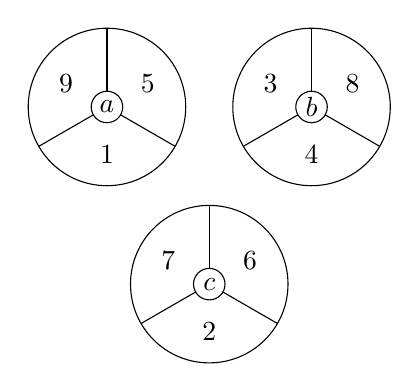
\begin{tikzpicture}
    \def \radius {1.5}
    \begin{scope}[shift={(150:\radius)}]
        \draw (0, 0) circle (1);
        \draw (0, 0) circle (0.2);
        \node at (0, 0) {$a$};
        \foreach \lineangle/\lblangle/\lbl in {90/150/9, 210/270/1, 330/30/5} {
            \draw (0, 0) +(\lineangle:.2) -- +(\lineangle:1);
            \path (0, 0) ++(\lblangle:.6) node {\lbl};
        }
    \end{scope}
    
    \begin{scope}[shift={(270:\radius)}]
        \draw (0, 0) circle (1);
        \draw (0, 0) circle (0.2);
        \node at (0, 0) {$c$};
        \foreach \lineangle/\lblangle/\lbl in {90/150/7, 210/270/2, 330/30/6} {
            \draw (0, 0) +(\lineangle:.2) -- +(\lineangle:1);
            \path (0, 0) ++(\lblangle:.6) node {\lbl};
        }
    \end{scope}

    \begin{scope}[shift={( 30:\radius)}]
        \draw (0, 0) circle (1);
        \draw (0, 0) circle (0.2);
        \node at (0, 0) {$b$};
        \foreach \lineangle/\lblangle/\lbl in {90/150/3, 210/270/4, 330/30/8} {
            \draw (0, 0) +(\lineangle:.2) -- +(\lineangle:1);
            \path (0, 0) ++(\lblangle:.6) node {\lbl};
        }
    \end{scope}
\end{tikzpicture}
\]

Es mejor ser el jugador $B$, sea $E_a, E_b, E_c$ el evento tal que $A$ elige el disco correspondiente y $B$ gana.

Si $A$ elige el disco
\begin{enumerate}
    \item[$a.$]
    y obtiene el siguiente valor $B$,
    \begin{enumerate}
        \item[9.] no puede ganar con ningún disco.
        \item[1.] gana siempre con el disco $c$.
        \item[5.] gana $\tfrac{2}{3}$ de las veces con el disco $c$.
    \end{enumerate}
    \[ P(E_a) = \tfrac{1}{3} * (0 + 1 + \tfrac{2}{3}) = \tfrac{5}{9} > \tfrac{1}{2} \]
    \item[$b.$]
    y obtiene el siguiente valor $B$,
    \begin{enumerate}
        \item[3.] gana $\tfrac{2}{3}$ de las veces con el disco $a$.
        \item[4.] gana $\tfrac{2}{3}$ de las veces con el disco $a$.
        \item[8.] gana $\tfrac{1}{3}$ de las veces con el disco $a$.
    \end{enumerate}
    \[ P(E_a) = \tfrac{1}{3} * (\tfrac{2}{3} + \tfrac{2}{3} + \tfrac{1}{3}) = \tfrac{5}{9} > \tfrac{1}{2} \]
    \item[$c.$]
    y obtiene el siguiente valor $B$,
    \begin{enumerate}
        \item[7.] gana $\tfrac{1}{3}$ de las veces con el disco $b$.
        \item[2.] gana siempre con el disco $b$.
        \item[6.] gana $\tfrac{1}{3}$ de las veces con el disco $b$.
    \end{enumerate}
    \[ P(E_a) = \tfrac{1}{3} * (\tfrac{1}{3} + 1 + \tfrac{1}{3}) = \tfrac{5}{9} > \tfrac{1}{2} \]
\end{enumerate}